
\section{Description of the Solution}
\subsection{Description of the software architecture}



Our software consists of three layers which are Input, Process, and Output layers. Data layer.

\vspace{\baselineskip}

The input layer is responsible for the preprocessing of examination plan files, enabling their utilization within the software.

\vspace{\baselineskip}

The process layer is responsible for analyzing the exam plan data to score, identifying conflicts, and visualizing data based on rules such as ensuring a one-day gap between exams.


\vspace{\baselineskip}

The output data is responsible for representing the scores, conflicts, and charts of every rule in a HTML file.

\FloatBarrier
\begin{figure}[ht]
    \centering
    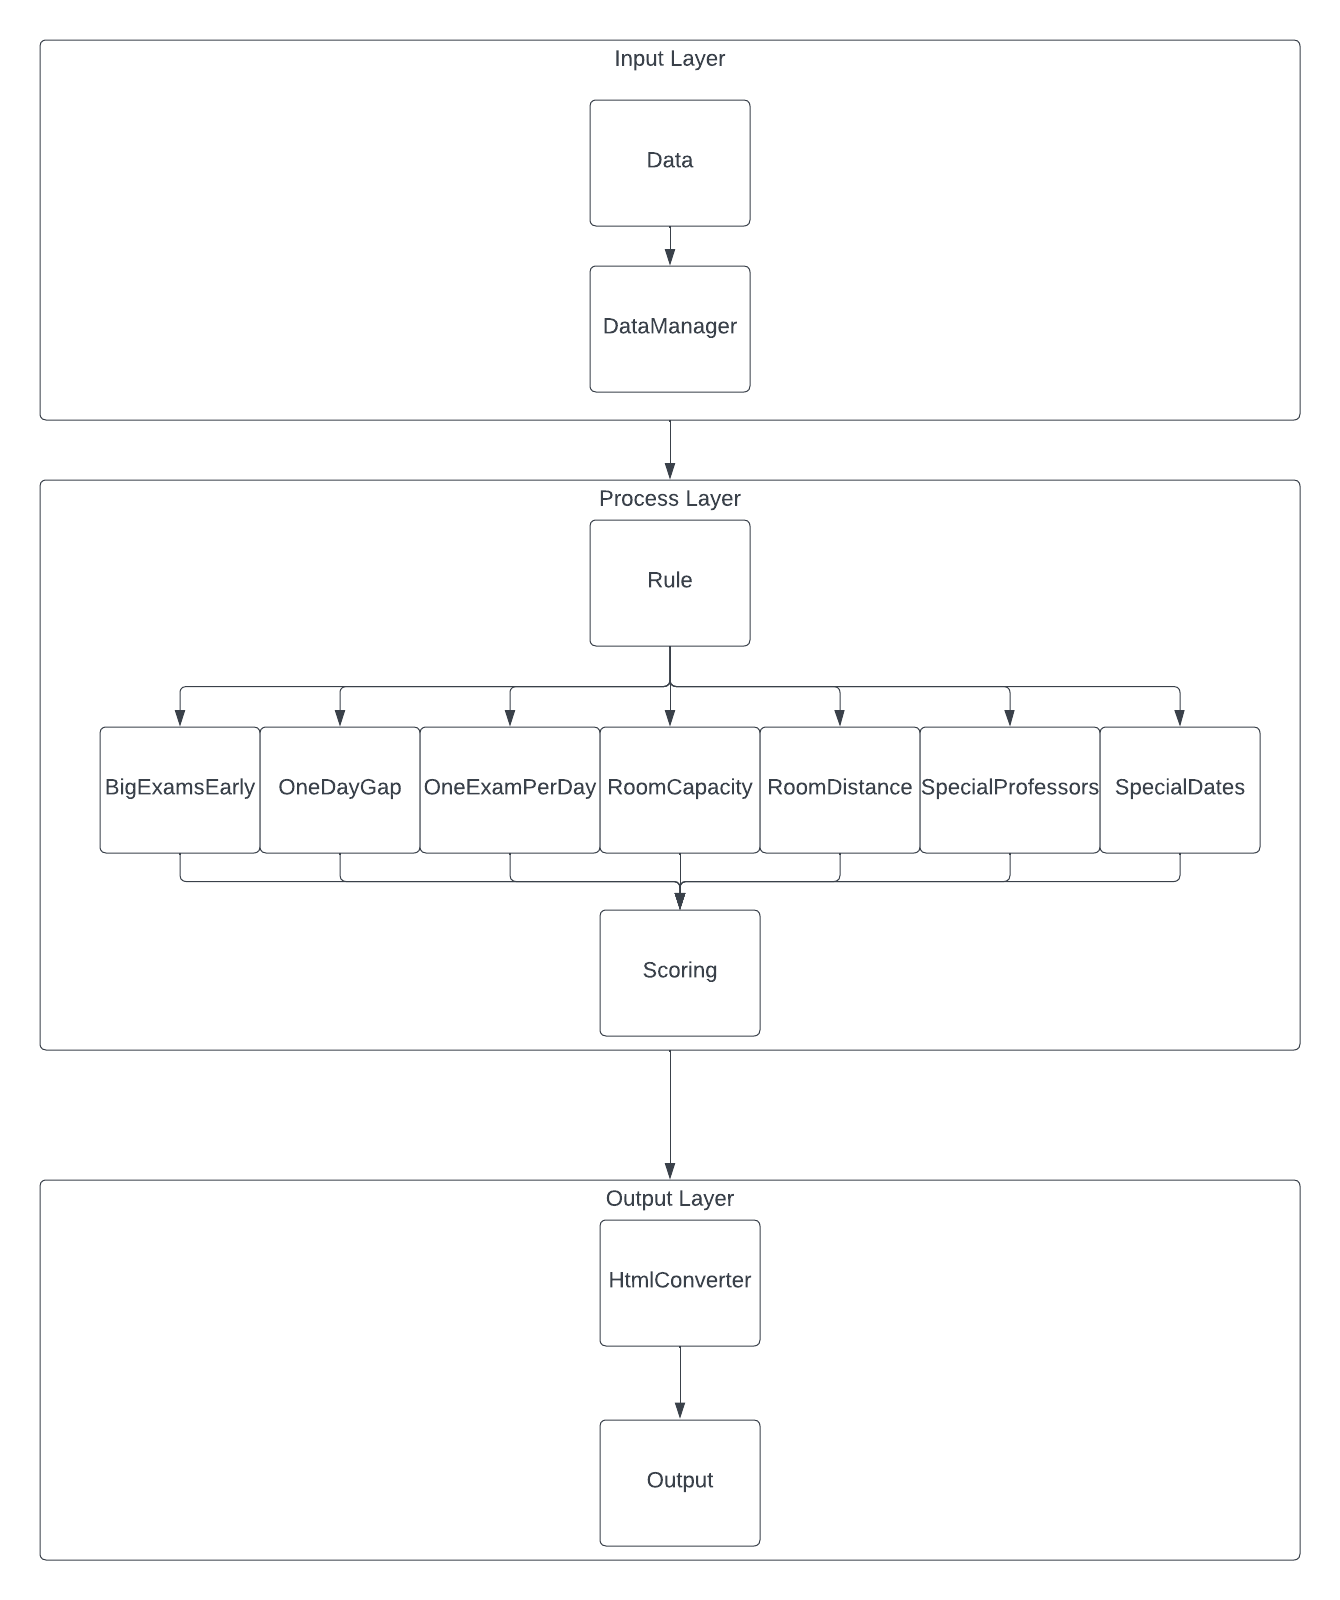
\includegraphics[width=160mm]{images/architecture.png}
    \caption{Architecture Design}
    \label{fig:entrance-screen}
\end{figure}
\FloatBarrier



\subsection{Overview and interaction of the components}


\subsubsection{Scoring Class}


\begin{itemize}
\item Scoring class interacts with the following rule classes: BigExamsEarly, OneExamPerDay, RoomCapacity, RoomDistance, SpecialProfessors, OneDayGap, SpecialDates.
\item This class is a wrapper for all of the rule classes. It is made to make it easy to access each of the components under one class.
\end{itemize}


\subsubsection{Data Class}


\begin{itemize}
\item The Data class is responsible for importing and organizing the input data from various files.
\item It can load different types of data such as CSV, JSON, and Excel. The following are the files that the Data class interacts with: \texttt{FIW\_Exams\_2022ws.xlsx}, \texttt{Pruefungsanmeldungen\_anonmous.csv}, \texttt{room\_distance\_matrix.xlsx}, \texttt{capacity.json}, \texttt{special\_dates.csv}, \texttt{specific\_professors.xlsx}.
\item It also splits and extracts relevant information from the loaded data and stores them as attributes and methods for further processing.
\item All of the rule classes interact with Data. It is a prerequisite for them to work.
\end{itemize}


\subsubsection{Output Class}


\begin{itemize}
\item Handles the generation and saving of output files.
\item Provides methods for saving the results as HTML files. These methods offers two different option either you can get a single result of one rule class or a summary list that includes all results.
\item Utilizes the HtmlConverter class to convert data into HTML format and print the output.
\end{itemize}


\subsubsection{HtmlConverter Class}


\begin{itemize}
\item Converts the processed data into HTML format for output representation.
\item Provides methods for creating HTML pages, and printing the HTML output.

\end{itemize}


\subsubsection{BigExamsEarly Class}


\begin{itemize}
\item Big exams should be held early in the exam period, and this class calculates the score and evaluates the exam plan based on the number of big exams and their scheduling time.
\end{itemize}


\subsubsection{OneExamPerDay Class}


\begin{itemize}
\item Verifies whether each student has only one exam scheduled per day.
\item Gives a penalty score while calculating the score of the exam plan based on the number of students who has multiple exams in a day.
\end{itemize}

\subsubsection{OneDayGap Class}


\begin{itemize}
\item This class calculates the score based on the absence of a one-day gap between exams for the same student.
\item basically identifies cases where there is no one-day gap between exams for the same student and calculates a general score for this rule by giving penalty based on the number of conflicts and also draws a plot showing the relationship between the number of conflicts and the score.
\end{itemize}

\subsubsection{RoomCapacity Class}


\begin{itemize}
\item Ensures that the assigned rooms can accommodate the number of students registered for each exam.
\item Computes the score by comparing the number of students with the room capacities for the each exam.
\end{itemize}

\subsubsection{RoomDistance Class}


\begin{itemize}
\item It search the rooms for each exam and if there is more than one room. It calculates the sub-scores of the distance between the relevant rooms.
\item This class has only score as its output.
\end{itemize}

\subsubsection{SpecialDates Class}


\begin{itemize}
\item This class is responsible for calculating the score for examiners, which are not able to come for the exam on a specific day.
\item Checks for conflicts between examiners' names and special dates in the \verb|special_dates_df|.
\item Import data class to reach \verb|special_dates_df| .
\item if there is a match, it adds the conflict information to the 'conflicts' list and makes a binary decision.
\item It returns a percentage score based on whether there is a conflict or not.
\end{itemize}

\subsubsection{SpecialProfessors Class}


\begin{itemize}
\item This class calculates special professors score based on the number of exams and the distance between those exam days that same professors supervise.

\end{itemize}

\subsubsection{Main Class}


\begin{itemize}
\item This class is responsible from the execution of the program and saving the various html results based on the demand.
\end{itemize}









\subsection{tasks of the component}
The components in the provided code and their interactions can be described as follows:

